\chapter{Introduction}
\label{introduction}

 \lhead{\emph{Introduction}} % Write in your own chapter title to set the page header 

\section{Health burden of coronary artery disease}
\label{healthburdenofcoronaryarterydisease}

Worldwide, coronary artery disease (CAD) is the most common cause of death, with around seven million people dying each year~\citep{steg_esc_2012}. In Europe, every sixth man and seventh woman will die from an acute myocardial infarction (AMI), or heart attack~\citep{widimsky_reperfusion_2009}. In developed countries, including the United Kingdom (UK), the incidence of myocardial infarction has been decreasing over the past 30 years~\citep{bilgi_interpretation_2012}, but there were still 125,245 inpatient episodes at National Health Service (NHS) facilities with a primary diagnosis of AMI in 2010\slash 11~\citep{british_heart_foundation_health_promotion_research_group_coronary_2012}. 

\section{Pathophysiology of myocardial infarction}
\label{pathophysiologyofmyocardialinfarction}

Coronary artery disease is almost always caused by atherosclerosis of the coronary arteries. This is a systemic, lipid (fat) driven immume\slash inflammatory disease of the medium and large arteries~\citep{falk_pathology_2003}. Over time (usually decades), atherosclerosis causes the formation of plaques; collections of lipids and cholesterol that accumulate in the intimal layer of
arteries, some of which attract macrophages (a type of white blood cell). The macrophages secrete protein dissolving enzymes and engulf the lipids, leaving behind a lipid-rich `necrotic core'. The interface between the plaque and the lumen of the artery is known as the fibrous cap.

Ruptured plaques are the most common cause of AMI~\citep{sakakura_pathophysiology_2013}, and typically involve a plaque with a thin fibrous cap~\citep{windecker_future_2013}. This rupture usually occurs during, or just after, a sympathetic nervous system trigger such as physical or sexual activity, anger, anxiety, work stress, temperature change or cocaine use~\citep{mittleman_physical_2011}. The exposed necrotic core is highly thrombogenic, leading to platelet aggregation and activation of the clotting cascade~\citep{curzen_what_2013}. Should the artery become completely occluded, blood proximal to the blockage will stagnate and may coagulate, extending the thrombosis along the artery and making subsequent reopening of the artery much more difficult~\citep{falk_pathology_2003}.

An occluded coronary artery will usually lead to myocardial cell death secondary to prolonged ischaemia, i.e. cause a myocardial infarction (MI). This process can begin in under 20 minutes, but complete necrosis of myocardial cells which have had their supplying coronary artery (or arteries) occluded, typically does not occur until 2--4 hours, and sometimes longer, have elapsed, depending upon the presence of collateral circulation, the pre-morbid state of the patient, the nature of the occlusion (intermittent or permanent) and the sensitivity of the myocytes to ischaemia, for example~\citep{thygesen_third_2012}. This provides an opportunity for timely salvage of the myocardium, improving heart function and reducing mortality, if blood flow can be restored~\citep{department_of_health_treatment_2008}. 

\section{The electrodcardiogram and AMI}
\label{theelectrodcardiogramandami}

The first step in the development of AMI is the onset of myocardial ischaemia, as oxygen delivery fails to meet demand. Clinically, this is typically identified from the patient history, presenting signs and symptoms, and interpretation of the 12-lead electrocardiogram (ECG). The ECG is a recording of the electrical activity generated by the cells of the heart, and is obtained by the placement of a number of electrodes around the heart, which provide different ‘views’ of this electrical activity~\citep{kligfield_recommendations_2007}. The resulting output on a screen or paper plots the voltage generated against time. Characteristic components of the ECG enable a clinician to recognise a number of medical conditions, including AMI. \autoref{ecgcomplex} shows the components of the ECG, including the ST segment and T wave, which are important in the recognition of a specific type of AMI, ST-segment elevation MI (STEMI)~\citep{thomas_garcia_12-lead_2000}. Ordinarily, the ST-segment is level with the baseline (typically measured at the level of the PR segment), as shown in the the normal 12-lead ECG in \autoref{ecgsegment}.

\begin{figure}[htbp]
\centering
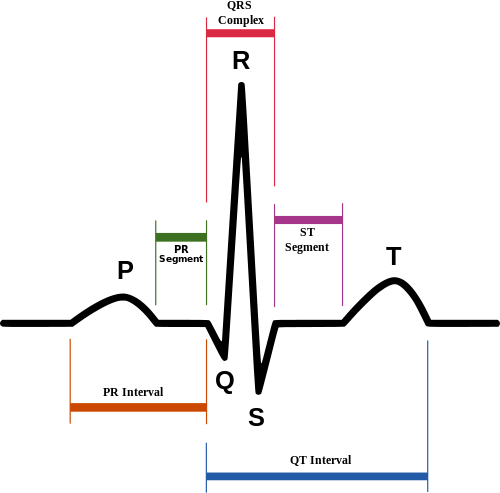
\includegraphics[keepaspectratio,width=0.6000\textwidth,height=0.75\textheight]{ECG.png}
\caption{The components of an ECG complex}
\label{ecgcomplex}
\end{figure}



\begin{figure}[htbp]
\centering
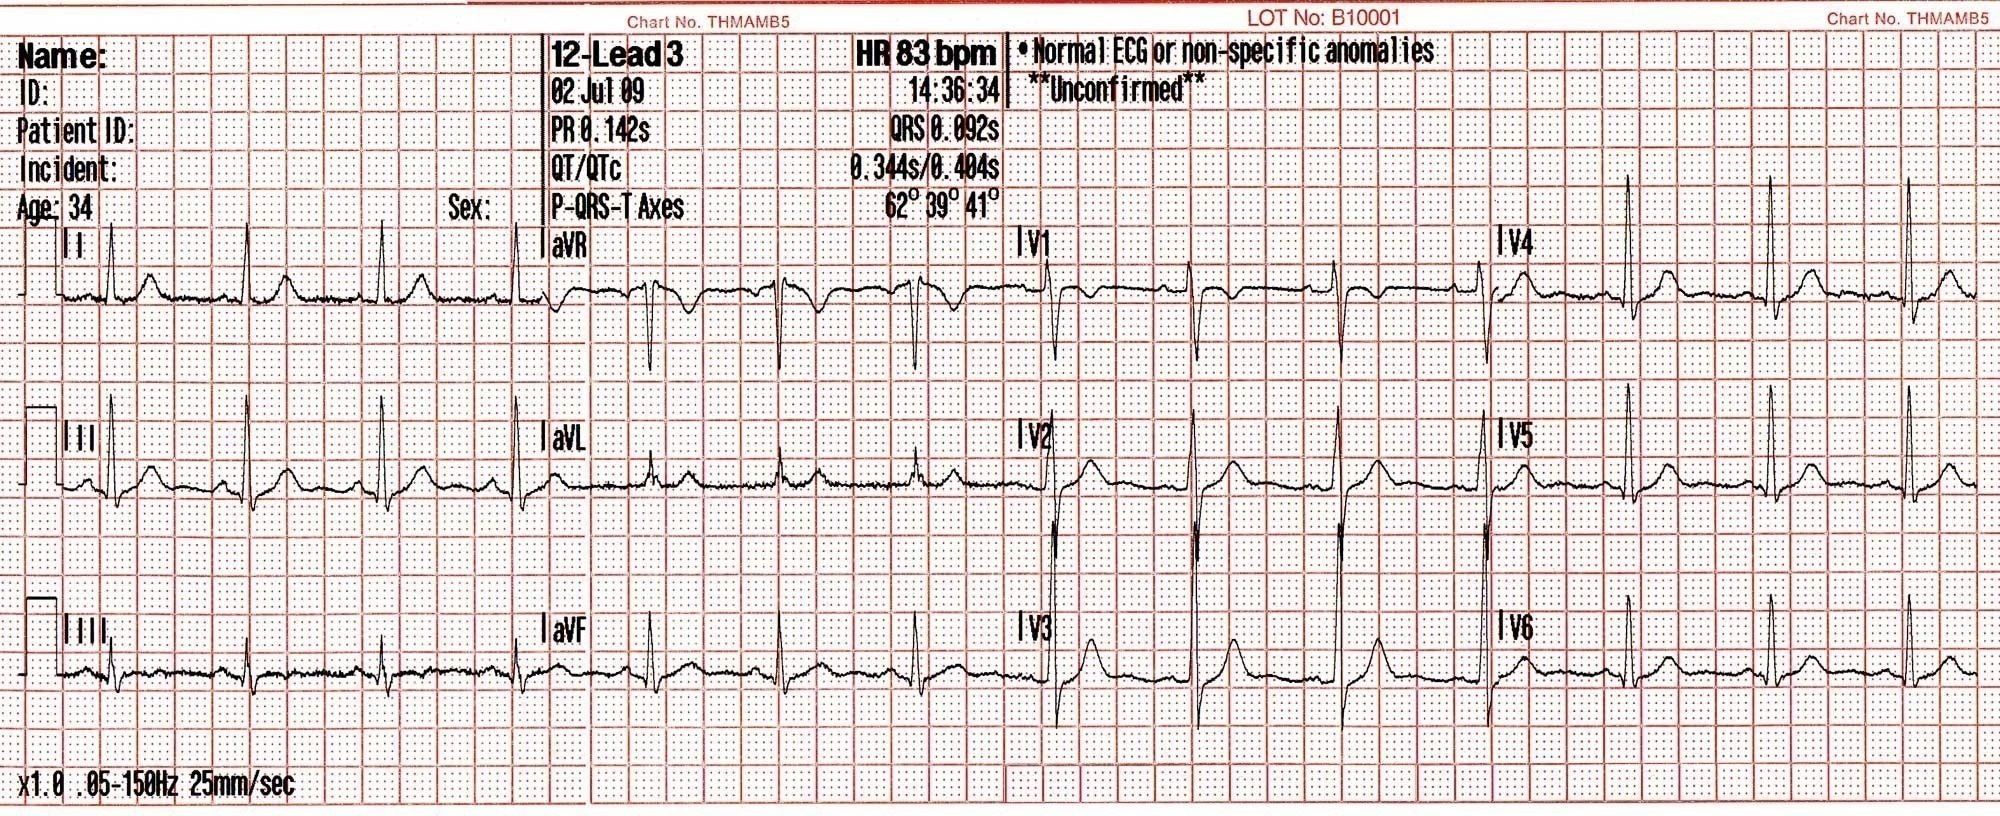
\includegraphics[keepaspectratio,width=0.9900\textwidth,height=0.75\textheight]{my-ecg-anon.jpg}
\caption{A normal 12-lead ECG}
\label{ecgsegment}
\end{figure}




During a period of myocardial ischaemia, myocardial injury often produces a characteristic rise in the ST-segment from the baseline. Criteria vary, but typically if the ST-segment rises 2mm or more in two or more leads looking at the same area of the heart, then the patient is said to be having a STEMI, even if myocardial necrosis has not yet occurred~\citep{association_of_ambulance_chief_executives_uk_2013}. \autoref{ecgstemi} shows an example of this ST-segment rise and the computer interpretation message, which is printed at the top of the 12-lead ECG.

\begin{figure}[htbp]
\centering
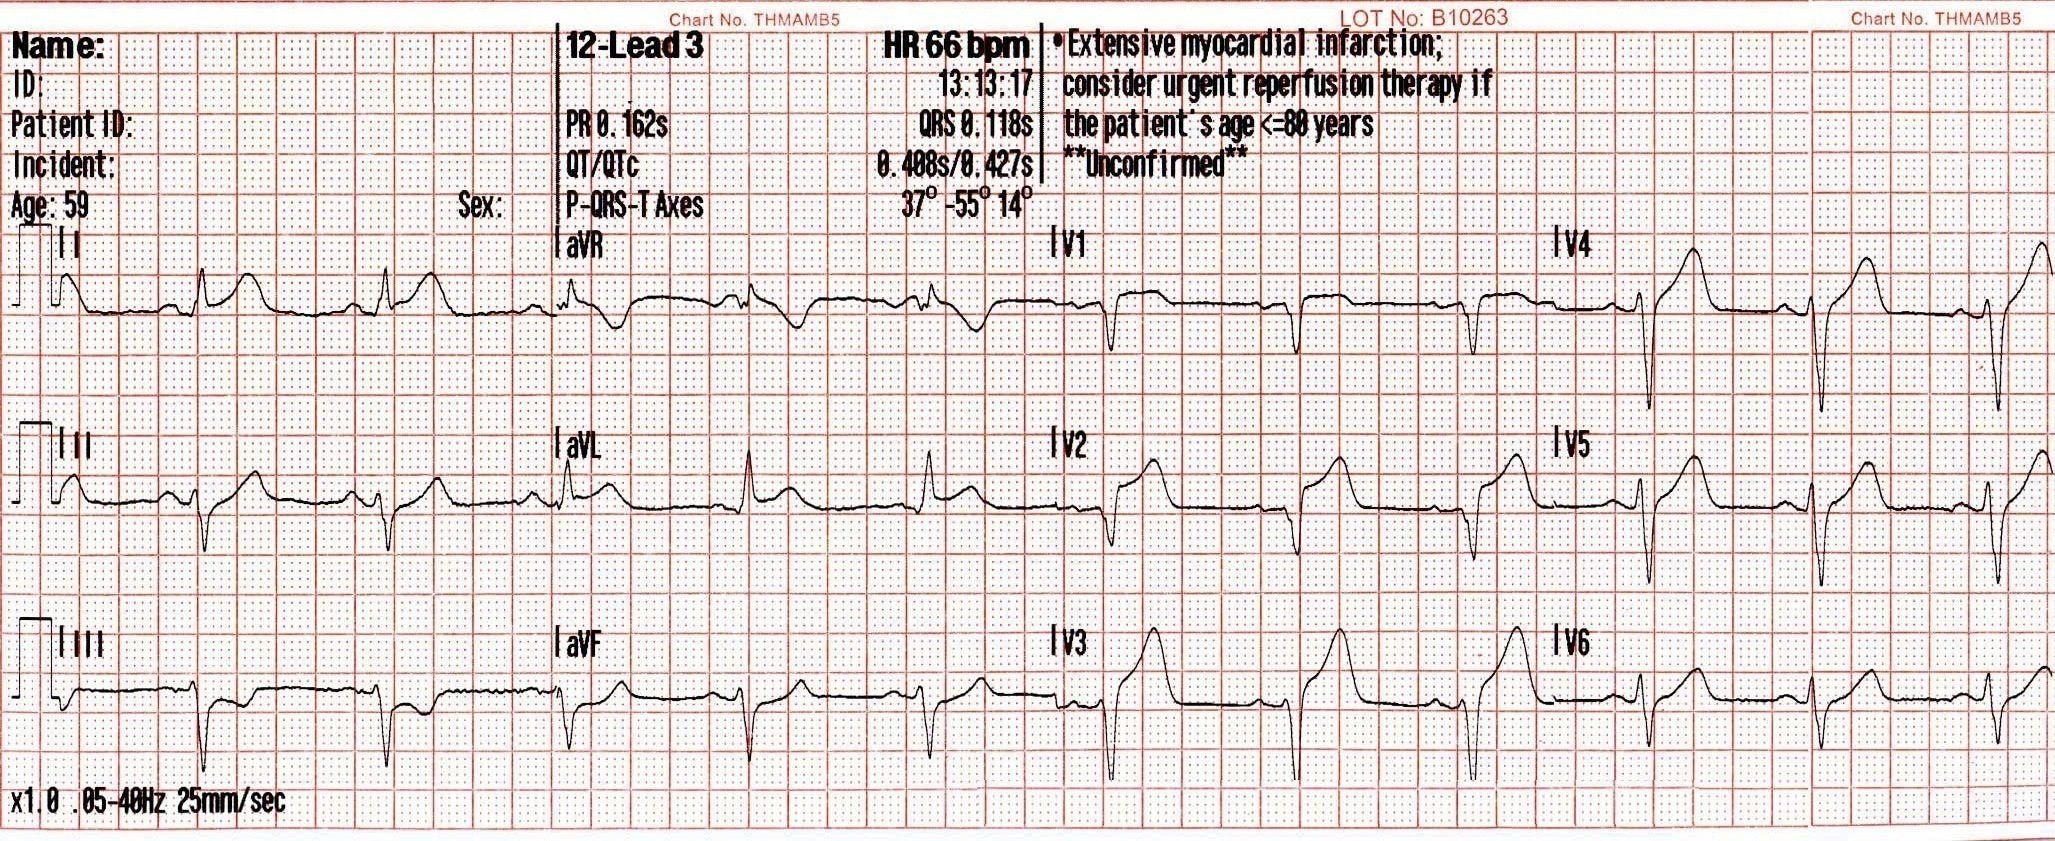
\includegraphics[keepaspectratio,width=0.9900\textwidth,height=0.75\textheight]{Sample-MI.jpg}
\caption{A 12-lead ECG with ST-segment elevation}
\label{ecgstemi}
\end{figure}



\section{Treatment of STEMI}
\label{treatmentofstemi}

Clinical trials have demonstrated a clear link between patient outcome and time to reperfusion in STEMI~\citep{department_of_health_treatment_2008}, which heightened interest in the prehospital recognition and treatment of STEMI. In 2001, prehospital thrombolysis was introduced, a technique previously only used in hospital, to chemically clear the blockage in the patient's coronary arteries. Initially, diagnosis was supported by the use of telemetry, whereby the ECG would be sent to the local hospital for diagnosis. Subsequent studies demonstrated that paramedics' diagnosis of STEMI was highly sensitive and specific~\citep{swor_prehospital_2006,feldman_real-time_2005}, leading some to question the need for telemetry with its associated costs and technical issues~\citep{woollard_limited_2005,keeling_safety_2003,johnston_paramedics_2006}. However, thrombolysis is associated with increased risk of bleeding, including haemorrhagic strokes, and is not always successful in clearing the affected coronary arteries. Fortunately, there is an alternative, mechanical clearance of coronary arteries with a balloon catheter and stent, collectively known as primary percutaneous coronary intervention (pPCI). In 2008, the National Infarct Angioplasty Project (NIAP) concluded that numerous international trials demonstrated reduced mortality and improved long-term outcome of pPCI compared with thrombolysis. However, this is time dependent, and delays beyond 90 minutes from when thrombolysis could have been administered, is considered to be point at which the benefit of pPCI is negated. In addition, NIAP also demonstrated that in order to achieve this, bypassing local hospitals in favour of a regional centre which had a cardiac catheter lab was the most effective (and cost-effective) method~\citep{department_of_health_treatment_2008}.

As with the early administration of thrombolysis, ambulance services now have an important role in minimising the time from a patient's call for professional help, to undergoing pPCI (the call-to-balloon time). In the UK, 95\% of STEMI patients are treated with pPCI, and 77.5\% of patients with STEMI are taken directly to the cardiac catheter labs by the ambulance service~\citep{ludman_national_2013}. The current European Society of Cardiology (ESC) guidelines for the management of patients presenting with STEMI, advocate the recording of a 12-lead ECG within 10 minutes of first medical contact, and direct transfer to a pPCI capable centre, if this is possible, within 120 minutes. If this is not possible, then the administration of thrombolysis should be achieved within 30 minutes~\citep{steg_esc_2012}. This guidance has been incorporated into the current UK ambulance service clinical guideline for the management of STEMI~\citep{association_of_ambulance_chief_executives_uk_2013}.

\section{Computer interpretation of ECGs}
\label{computerinterpretationofecgs}

Since Augustus Waller first demonstrated the measurement of electrical current produced by the human heart in 1887 (\autoref{jimmie})~\citep{waller_demonstration_1887,herring_ecg_2006}, ECG recording fidelity has improved considerably, as has the portability of the hardware required to produce the waveforms. 

\begin{figure}[htbp]
\centering
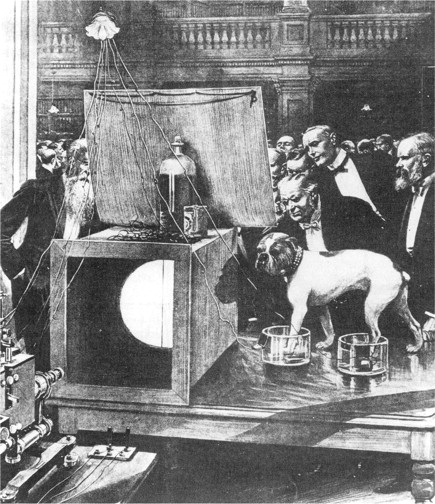
\includegraphics[keepaspectratio,width=0.5000\textwidth,height=0.75\textheight]{bulldog.jpg}
\caption{Waller demonstrating at the Royal London Society with his bulldog Jimmie}
\label{jimmie}
\end{figure}



However, recording the ECGs is just the first step, since they also require interpretation. Since skilled personnel are not universally available, computers have been seen as a possible solution. In the 1960s, computer interpretation of ECGs was introduced, although this was typically only available at larger hospitals with large, dedicated computers~\citep{willems_computer_1981}. Today, computer interpretation of ECGs is possible at the patient's side, thanks to the increased power and reduced size of computers.

In order to interpret an ECG, a computer needs to complete five steps~\citep{kligfield_recommendations_2007}:

\begin{enumerate}
\item Obtaining and filtering the signal

\item Identifying and sorting complexes in order to create an average (typically median) complex for each lead

\item Recognising the waveform and identifying the onset and offset of a single complex

\item Extracting features from complexes and measuring amplitudes and intervals

\item Utilising heuristic or statistical methods to allocate diagnoses.

\end{enumerate}

\subsection{ECG standards}
\label{ecgstandards}

In order to introduce a standard performance benchmark for the first four steps, a Common Standard for Quantitative Electrocardiography (CSE) database was created in the late 1980s (and finalised in 1990). This consists of 1220 calibrated ECGs which are provided to manufacturers to test their ECG hardware and software~\citep{willems_comparison_1991,willems_diagnostic_1991}. These ECGs were subsequently incorporated into the International Electrotechnical Commission standard IEC 60601--2--51 (superseded by IEC 60601--2--25 ed2.0 in 2011), which also includes acceptable tolerances in mean and standard deviation differences from the published measurements~\citep{international_electrotechnical_commission_medical_2011}. In addition, there are also standards relating to the messages produced by the computer interpretation algorithm. Examples of these are shown in \autoref{bethesda}~\citep{rautaharju_task_1978}.

\begin{table}[htbp]
\begin{minipage}{\linewidth}
\setlength{\tymax}{0.5\linewidth}
\centering
\small
\caption{ECG computer interpretation statements}
\label{bethesda}
\begin{tabulary}{\textwidth}{@{}CLL@{}} \toprule
\textbf{Type}&\textbf{Description}&\textbf{Example}\\
\midrule
A&Diagnosis of an anatomical lesion relating to pathophysiological state&Interior infarct\\
B&Diagnosis of electrophysiological changes&Left bundle branch block\\
C&Descriptive ECG features&Nonspecific ST abnormality\\

\bottomrule

\end{tabulary}
\end{minipage}
\end{table}


\subsection{Computer interpretation algorithms}
\label{computerinterpretationalgorithms}

Probably the most ubiquitous ECG interpretation algorithm in use by UK ambulance personnel is the General Electric (GE) Healthcare Marquette 12SL ECG analysis program~\citep{ge_healthcare_marquette_2010}. This is a heuristic algorithm, utilising experience-based, deterministic rules that incorporate measurements from the median waveform into a decision tree and boolean combinations of criteria~\citep{kligfield_recommendations_2007}.

Other algorithms adopt alternative approaches, such as statistical methods, which generate probability statements. An example is the acute cardiac ischaemia time-insensitive predictive instrument (ACI-TIPI)~\citep{selker_use_1998}. At least one algorithm in use by prehospital healthcare professionals utilises algorithms trained using artificial neural networks~\citep{eggers_artificial_2007}, although in practice, these have been found to work better if combined with more traditional, deterministic, methods rather than as a standalone method~\citep{physio_control_glasgow_2009-1}. 

\subsection{Validation of ECG algorithms}
\label{validationofecgalgorithms}

Irrespective of the method used by the ECG interpretation algorithm, there is a need for training and testing in order to validate its use more generally. This typically consists of training the algorithm on databases containing ECGs with specific, often single, pathophysiologies, for example an MI or a specific arrhythmia. Subsequent testing usually utilises much larger ECG databases, containing a wide spectrum of ECG electrophysiologies, in order to calculate sensitivity and specificity statistics. The gold standard varies, depending on what characteristic is being tested. For example, the expert opinion of a cardiologist might be appropriate for conditions such as arrhythmias whereas, in acute coronary syndromes, it is more typical for cardiac enzymes or angiography confirmation of diagnosis to be used~\citep{ge_healthcare_marquette_2008,ge_healthcare_marquette_2007}. 

\section{Recognition of STEMI by paramedics}
\label{recognitionofstemibyparamedics}

Timely diagnosis and appropriate management of patients with STEMI depends on accurate interpretation of the 12-lead ECG by paramedics. However, since only 4--6\% of chest pain calls to emergency services are actually acute coronary syndromes, this is not always straightforward~\citep{deakin_does_2006}. Thus, initial and ongoing training in the accurate acquisition and interpretation of 12-lead ECGs by paramedics, is important~\citep{ting_implementation_2008,ducas_transmit_2012}.

There is little published literature about the training provided to UK ambulance personnel in relation to ECG interpretation. The most credible is arguably a 2001 technology appraisal process document, authored by the Joint Royal College Ambulance Liaison Committee (JRCALC) and the Ambulance Services Association (ASA), which set out a suggested syllabus for a prehospital thrombolysis course~\citep{the_joint_royal_colleges_ambulance_liaison_committee_pre-hospital_2001}. This itself, was based on existing courses being run at the time by four ambulance services and included the following topic areas:

\begin{enumerate}
\item ECG acquisition

\item Components of a `normal' ECG

\item Arrhythmias

\item Coronary artery disease

\item The ECG in coronary artery disease

\item Management of MI including thrombolytics and other drugs.

\end{enumerate}

Two courses were created by pharmaceutical companies who manufactured thrombolysis drugs, namely Fast Track to Thrombolysis by Roche, and Thrombolysis Up Front by Boehringer Ingelheim. These courses were provided free of charge to UK ambulance services, and although there are no national statistics regarding the utilisation of such course material, Thrombolysis Up Front was used by every UK ambulance service at that time~\citep{watts_thrombolysis_2013}.

In the absence of telemetry, computer aided interpretation of the 12-lead ECG is an attractive option, and is available on all ECG monitors carried by UK ambulance services (although at extra cost). Depending on the study, computer interpretation alone is 58--78\% sensitive and 90--100\% specific, with false positive rates varying between 19--39\%~\citep{bhalla_prehospital_2013,clark_automated_2010,youngquist_comparison_2008}. Most studies consist of a mixture of paramedic and computer interpretation combined, either embedded in a protocol (usually requiring paramedic and computer agreement), or available for the paramedic to optionally utilise as a diagnostic tool. Sensitivities in this instance fall in the range 68--99.6\%, specificities 68--97\% and false positive rates 12--40\%~\citep{cantor_prehospital_2012,ducas_transmit_2012,ioannidis_accuracy_2001,mixon_retrospective_2012,ting_abstract_2009,young_paramedics_2011}. However, with the exception of one study, in which the computer interpretation was deliberately switched off, it is difficult to unpick what effect the computer interpretation, and the paramedic's own diagnostic skills, contribute to the figures mentioned. If it is the case that computer interpretation is adversely affecting accurate interpretation of the ECG, then it can be switched off. It may be the case, that the initial, and continuing, education of paramedics is the key. However, it is also possible that maintaining the status quo (i.e. a combination of paramedic and computer interpretation) is the best option. 

\section{Consequences of false negatives and positives}
\label{consequencesoffalsenegativesandpositives}

In contrast to early studies examining paramedics' safe administration of thrombolysis, false-positive rates for pPCI referral, have been reported to be 20--31\%~\citep{young_paramedics_2011,davis_positive_2007,rokos_appropriate_2010,swan_factors_2009}, possibly due to poor ECG recording, mis-interpretation of the ECG and\slash or the perception that pPCI is less risky than administering thrombolytics~\citep{smith_st-elevation_2001}. Inappropriate referral to pPCI centres has potential cost implications, may contribute to staff burnout, particularly for hospital staff who are called in from home out-of-hours, and result in longer patient transport times to a regional pPCI centre, rather than the local emergency department (ED), which is associated with an increased risk of mortality~\citep{nicholl_relationship_2007}.

False negatives are equally undesirable, since failure to identify and appropriately manage patients with STEMI, is more likely to result in delayed time to reperfusion, with the subsequent negative impact on mortality and morbidity~\citep{department_of_health_treatment_2008}. However, existing research has not explored this in any detail. Work on thrombolysis perhaps unsurprisingly focussed on ensuring the patients paramedics choose to thrombolyse had been selected appropriately, ignoring those who may have been inappropriately missed~\citep{khan_paramedic-led_2009,pitt_prehospital_2002,smith_paramedic_2010}. In addition, research examining the prehospital activation of cardiac catheter labs, perhaps unsurprisingly, focussed on false positive rates and the impact this would have on pPCI services. However, only recruiting participants on a pPCI pathway meant that none of the studies were able to identify patients who were missed (with the exception of the Ting study~\citep{ting_abstract_2009}, which did record patients who had been taken to the ED at the study hospital). 

\section{Research focus}
\label{researchfocus}

The Recognition of STEMI by Paramedics and the Effect of Computer inTerpretation (RESPECT) aims to answer the following research question:

\begin{quote}

Do computer interpretation messages have an effect on paramedics' diagnosis of STEMI from a 12-lead ECG?
\end{quote}
